%Version 3.1 December 2024 -- Springer Nature LaTeX template (sn-jnl), official package
%downloaded from resource-cms.springernature.com on 2026-10-23 (see report/final/README.md).
%Numbered Math and Physical Sciences reference style.
\documentclass[pdflatex,sn-mathphys-num,twocolumn,lineno]{sn-jnl}

\usepackage{graphicx}%
\usepackage{multirow}%
\usepackage{amsmath,amssymb,amsfonts}%
\usepackage{amsthm}%
\usepackage{mathrsfs}%
\usepackage[title]{appendix}%
\usepackage{xcolor}%
\usepackage{textcomp}%
\usepackage{manyfoot}%
\usepackage{booktabs}%
\usepackage{array}%
\usepackage{tabularx}%
\usepackage{xurl}%
\usepackage{tikz}%
\usepackage{stfloats}%
\usetikzlibrary{arrows.meta,positioning,fit,calc,backgrounds}%
\geometry{reset,paperwidth=210mm,paperheight=297mm,left=13.5mm,right=13.5mm,top=20mm,bottom=18mm,headheight=5.5pt,headsep=5.6mm,footskip=8mm,twocolumn,columnsep=6.3mm}
\setlength\columnsep{6.3mm}
\setcounter{dbltopnumber}{3}
\renewcommand\dbltopfraction{0.9}
\renewcommand\dblfloatpagefraction{0.6}
\renewcommand\textfraction{0.1}
\newlength\origtw
\setlength\origtw{372pt}
\newenvironment{widefigure}[1][tbp]{\begin{figure*}[#1]\centering\begin{minipage}{\origtw}\setlength\textwidth{\origtw}\setlength\columnwidth{\origtw}}{\end{minipage}\end{figure*}}
\newenvironment{widetable}[1][tbp]{\begin{table*}[#1]\centering\begin{minipage}{\origtw}\setlength\textwidth{\origtw}\setlength\columnwidth{\origtw}\begin{center}\begin{threeparttable}\tablebodyfont\renewcommand\footnotetext[2][]{{\removelastskip\vskip3pt\let\tablebodyfont\tablefootnotefont\hskip0pt\if!##1!\else{\smash{$^{##1}$}}\fi##2\par}}}{\end{threeparttable}\end{center}\end{minipage}\end{table*}}


\theoremstyle{thmstyleone}%
\newtheorem{theorem}{Theorem}%

\raggedbottom
\emergencystretch=3em
\sloppy

% Values from the audit runs (see report/final/evidence_ledger.md).
\newcommand{\LATMS}{20.9\,ms}
\newcommand{\LATIQR}{20.2--21.9\,ms}

% ---------------------------------------------------------------------------
% Evidence links. Every code and result link is pinned to the audited commit.
% \ev{path#anchor}{shown text}: the shown text is typeset as a breakable URL.
% ---------------------------------------------------------------------------
\newcommand{\repo}{https://github.com/not-good-keeper/compact-vit-sign-language/blob/v1.0}
\newcommand{\treeurl}{https://github.com/not-good-keeper/compact-vit-sign-language/tree/v1.0}
\newcommand{\ev}[2]{\href{\repo/#1}{\nolinkurl{#2}}}
\newcommand{\evdir}[2]{\href{\treeurl/#1}{\nolinkurl{#2}}}
\newcommand{\new}[1]{\nolinkurl{#1}}
% Source note under a figure: one short paragraph, same style as a table footnote.
\newcommand{\src}[1]{\par\vspace{3pt}{\footnotesize\raggedright\setlength{\parindent}{0pt}#1\par}}
\newcolumntype{L}[1]{>{\raggedright\arraybackslash\hspace{0pt}}p{#1}}
\newcolumntype{Y}{>{\raggedright\arraybackslash\hspace{0pt}}X}

\definecolor{cA}{HTML}{2a78d6}
\definecolor{cB}{HTML}{eb6834}
\definecolor{cC}{HTML}{1baf7a}
\definecolor{cD}{HTML}{eda100}
\definecolor{ink2}{HTML}{52514e}
\definecolor{panel}{HTML}{f3f2ef}
\tikzset{
  box/.style={draw=ink2, rounded corners=2pt, align=center, font=\footnotesize, inner sep=3pt, minimum height=7mm, fill=white},
  stage/.style={box, fill=panel},
  arr/.style={-{Stealth[length=2.2mm]}, draw=ink2, line width=0.6pt},
  lab/.style={font=\scriptsize, text=ink2, align=center},
}


\usepackage{xr-hyper}
\externaldocument{supp}

\begin{document}

\title[Compact factorised ViT for isolated ISL words]{ISL-ViT-Tiny: A Compact Factorised Vision Transformer for Isolated-Word Indian Sign Language Recognition, Evaluated on Held-Out Recording Sessions}

\author[1]{\fnm{Nethi} \sur{Kushala Kumar}}
\author[1]{\fnm{Yalamanchi} \sur{Kushal}}
\author*[1]{\fnm{Bagyammal} \sur{Thirumurthy}}\email{t\_bagyammal@cb.amrita.edu}
\author[1]{\fnm{Dhrusheek} \sur{Rishi Menon}}

\affil[1]{\orgdiv{Department of Computer Science and Engineering}, \orgname{Amrita School of Computing, Amrita Vishwa Vidyapeetham}, \orgaddress{\city{Coimbatore}, \country{India}}}

\abstract{Isolated-word recognition of Indian Sign Language (ISL) on a wearable device needs a small model whose accuracy is measured on recordings it has not seen. We present ISL-ViT-Tiny, a factorised spatio-temporal Vision Transformer (ViT) that reads three detected crops per frame (left hand, right hand, face) over 16 frames, adds 21 hand-joint landmarks per hand to the hand tokens, and is trained on the Indian Lexicon Sign Language Dataset (INCLUDE; 262 words) after masked-image pretraining on iSign. Evaluation holds out whole recording sessions, identified from camera clip counters. On 472 held-out clips of the 50 deployed words, with predictions restricted to those words and six-view test-time augmentation, the released 4-bit model (2,069,700 bytes; 3,894,214 parameters) reaches 85.9\% mean top-1 accuracy over three seeds and 96.4\% top-5. Hand landmarks add 12.8 points over pixels alone; quantisation-aware training keeps accuracy within seed noise of full precision. Trained on INCLUDE's own split, the same model scores 97.9\% (INCLUDE-50) and 98.8\% (262 words), against previously reported 94.5\% and 85.6--97.8\%; a matched pixel-only configuration falls from 98.5\% on a random-video split to 70.1\% on held-out sessions. A learned super-resolution front end raises 180p accuracy from 61.0\% to 76.0\%.}

\keywords{Indian Sign Language recognition, Vision Transformer, hand landmarks, 4-bit quantisation, evaluation protocol, super-resolution GAN}

\maketitle

% ===========================================================================
\section{Introduction}\label{sec:intro}
% ===========================================================================

Indian Sign Language (ISL) is the primary language of a large Deaf community in India; the authors of the Indian Lexicon Sign Language Dataset (INCLUDE) cite more than five million users~\cite{sridhar2020include}. An automatic recogniser for isolated ISL words could support communication with non-signers, and a camera on a pair of smart glasses is one place such a recogniser could run. That target sets two requirements that pull against each other. The network must fit a memory and compute budget far below that of standard video models, and its reported accuracy must describe what happens when the signer, room and lighting differ from the training recordings.

The second requirement is the harder one to meet with public ISL data. INCLUDE, the main labelled word-level corpus, contains 4,287 videos of 263 words recorded by experienced signers~\cite{sridhar2020include}; the copy used here has 4,257 usable clips of 262 words. A word has a median of 15 clips, many of them back-to-back takes of the same signer in the same session. A random split of such data puts near-identical takes on both sides of the train/test boundary, so a high score can reflect recognition of the recording rather than of the sign. The problem is not specific to sign language: Kapoor and Narayanan document train--test leakage across machine-learning-based science~\cite{kapoor2023leakage}. Within sign language, the Ankara University Turkish Sign Language dataset (AUTSL) reports 95.95\% for its baselines on random splits and 62.02\% on its user-independent split~\cite{sincan2020autsl}. Published INCLUDE results of 85.6\% (263 words) and 94.5\% (INCLUDE-50)~\cite{sridhar2020include}, and 93.5 to 97.8\% for pose-based models~\cite{selvaraj2022openhands,patra2024hwgat}, were obtained on the dataset's own split. Section~\ref{sec:res:protocol} measures how much splits that mix recordings inflate accuracy on this corpus, and Section~\ref{sec:res:sota} trains the method of this paper on the dataset's own split and compares on the same test clips.

Transformer video models~\cite{arnab2021vivit,bertasius2021timesformer} and pose-based sign recognisers~\cite{bohacek2022spoter,jiang2021samslr,selvaraj2022openhands} give strong results on sign data, and recent work targets edge hardware~\cite{lamaakal2026tinymslr,venkatappa2026kannada}. In the sources we reviewed (Section~\ref{sec:related}) we did not find an ISL word recogniser that reports, in one place, a hard size budget, a measured quantisation cost and a split that holds out whole recording sessions.

The contributions are:
\begin{enumerate}
\item A task-specific compact recogniser: a factorised spatial-then-temporal Transformer over hand and face crops, with crop position, detection status and normalised hand-joint features added to the crop tokens (Section~\ref{sec:method:model}), sized and quantised to a 2\,MB budget.
\item Controlled measurements on one fixed test set: the landmark stream (+12.8 points, paired $p\le 5\times10^{-9}$ in each seed), post-training versus quantisation-aware 4-bit compression, temporal length, crop resolution and training duration (Section~\ref{sec:results}).
\item A recording-session-aware evaluation built from capture identifiers, with a matched measurement of how much a random split inflates accuracy (about 28 points for one configuration) (Section~\ref{sec:method:eval}), and a comparison with published INCLUDE results on the dataset's own split, on the same test clips (Section~\ref{sec:res:sota}).
\item A controlled super-resolution study that separates the benefit of a learned upscaler from the benefit of the adversarial loss (Section~\ref{sec:res:gan}).
\end{enumerate}

% ===========================================================================
\section{Related work}\label{sec:related}
% ===========================================================================

\paragraph{ISL datasets and recognisers.} INCLUDE~\cite{sridhar2020include} is the reference labelled corpus for isolated ISL words; its best model, a pretrained feature extractor and encoder with a trained decoder, reached 85.6\% on 263 words and 94.5\% on the 50-word subset. The Corpus for Indian Sign Language Recognition (CISLR)~\cite{joshi2022cislr} has a vocabulary of about 4,700 words with roughly 1.5 videos per word, so its authors frame recognition as a one-shot task; their prototype baseline, built on features from an Inflated 3D ConvNet (I3D), reached 16.81\% top-1 on CISLR v1.0-a. iSign~\cite{joshi2024isign} provides a large collection of ISL video--sentence pairs and benchmark tasks. Recent ISL systems include a conversational agent that combines a convolutional neural network (CNN) with a ViT reporting 97.5\% accuracy under optimised conditions on a domain-specific dataset~\cite{nedungadi2025vit} and a two-handed dynamic ISL recogniser~\cite{govindharajalu2025isl}; Damdoo and Kumar survey the field~\cite{damdoo2025survey}.

\paragraph{Video and pose models for sign recognition.} The ViT~\cite{dosovitskiy2021vit} and the training procedure of the data-efficient image Transformer (DeiT)~\cite{touvron2021deit} made patch-token models practical on modest datasets. For video, the Video Vision Transformer (ViViT)~\cite{arnab2021vivit} studies variants that factorise spatial and temporal attention, and TimeSformer~\cite{bertasius2021timesformer} compares divided space--time attention with joint attention. Sign Language Transformers~\cite{camgoz2020slt} applied Transformers to continuous recognition and translation. Pose-based recognisers operate on body and hand keypoints: the Sign Pose-based Transformer (SPOTER)~\cite{bohacek2022spoter} normalises hand poses in a local coordinate frame and reports 63.18\% on WLASL100, the 100-word subset of the Word-Level American Sign Language dataset (WLASL); Skeleton Aware Multi-modal Sign Language Recognition (SAM-SLR)~\cite{jiang2021samslr} fuses a skeleton stream, processed by graph convolutional networks (GCNs), with red--green--blue (RGB) and depth streams; SignBERT~\cite{hu2021signbert} pretrains a hand-model-aware representation in the manner of Bidirectional Encoder Representations from Transformers (BERT); OpenHands~\cite{selvaraj2022openhands} releases pose-based models for six sign languages, built on long short-term memory (LSTM) networks, BERT, a spatial-temporal GCN (ST-GCN) and a sign-language GCN (SL-GCN), and reports 93.5\% (SL-GCN) on INCLUDE, rising to 94.7\% with self-supervised pretraining. HWGAT~\cite{patra2024hwgat}, a hierarchical windowed graph attention network over MediaPipe keypoints released as a preprint, reports 97.67\% on INCLUDE, and 97.79\% after pretraining on a larger ISL word corpus. Our model combines the two families: pixels of detected regions, plus hand landmarks from MediaPipe~\cite{lugaresi2019mediapipe,zhang2020mphands} added to the visual tokens rather than processed by a separate graph network.

\paragraph{Compact models and quantisation.} Integer quantisation with simulated rounding during training~\cite{jacob2018quant} and the straight-through gradient estimator~\cite{bengio2013ste} are the standard basis of quantisation-aware training; Nagel et al. review post-training and quantisation-aware methods~\cite{nagel2021whitepaper}. Q-BERT~\cite{shen2020qbert} and GPTQ~\cite{frantar2023gptq} give each block of weights its own scale (group-wise scaling). For sign recognition at the edge, TinyMSLR~\cite{lamaakal2026tinymslr} reports fewer than 2.7\,M parameters and 7.2\,MB on a 20-class isolated-sign benchmark built from two corpora with a signer-independent protocol, and a Kannada Sign Language study~\cite{venkatappa2026kannada} deploys quantised LSTM and Transformer models on a smartphone.

\paragraph{Evaluation protocols.} WLASL~\cite{li2020wlasl} collects more than 2,000 words from over 100 signers, and AUTSL~\cite{sincan2020autsl} publishes a user-independent benchmark split and reports the random-versus-user-independent gap quoted in Section~\ref{sec:intro}. INCLUDE ships without signer identifiers; the protocol in Section~\ref{sec:method:eval} reconstructs recording sessions from the camera's running clip counter.

\paragraph{Super-resolution for recognition.} SRGAN, a super-resolution generative adversarial network (GAN)~\cite{ledig2017srgan}, its enhanced version ESRGAN~\cite{wang2018esrgan} and Real-ESRGAN~\cite{wang2021realesrgan} sharpen upscaled images by training the generator against a discriminator~\cite{goodfellow2014gan}. Blau and Michaeli show that perceptual quality and distortion measures such as peak signal-to-noise ratio (PSNR) trade off against each other~\cite{blau2018pd}. Whether super-resolution helps a downstream task is an empirical question: Dai et al. examined it for several vision tasks~\cite{dai2016srhelpful}, and Haris et al. trained super-resolution with a detection loss~\cite{haris2018taskdriven}. Our study asks the narrower question of what the adversarial term adds to learned upscaling for a frozen sign recogniser.

Supplementary Table~\ref{tab:lit} places the closest works beside this work. Numbers are as reported by each paper; datasets, vocabularies and splits differ, so the column is not a ranking.

% ===========================================================================
\section{Proposed methodology}\label{sec:method}
Figure~\ref{fig:archpipe} shows the end-to-end pipeline. For each clip, 32 frames are sampled, a landmark detector locates the hands and face, six 16-frame views are drawn, and the 4-bit classifier scores every view; pretraining, supervised training and quantisation-aware training run once, offline, before deployment. Sections~\ref{sec:method:data} to~\ref{sec:method:metrics} describe these stages in turn.

\begin{figure*}[tp]
\centering
\includegraphics[width=\textwidth]{figures/fig_pipeline_architecture.pdf}
\caption{End-to-end pipeline. The four upper panels run for every clip; the band below runs once, offline. Funnels are learned models, offset squares are stacks of frames and small bar charts are probability vectors. (1)~\textit{Frames}: 32 frames are sampled uniformly. Frames shorter than 720 pixels are enlarged by bicubic interpolation or, as an option, by the $\times4$ super-resolution generator; taller frames are area-downsampled; all are letterboxed to $1280\times720$. (2)~\textit{Landmarks}: a holistic detector, rebuilt for every clip, returns pose, face and hand landmarks, and the face and hand boxes are squares around them enlarged 1.3 and 1.5 times. The dashed box is the path for a missing hand: a region of 2.8 forearm lengths around the wrist is upsampled to 256 pixels and passed to a single-hand detector, and if that also fails the nearest real box is reused and flagged as interpolated. That flag is the detection indicator of Fig.~\ref{fig:archmodel}. (3)~\textit{Views}: one frame is taken from each of 16 equal segments at three phase offsets (ticks), and each selection is also mirrored with the hand streams swapped, giving six views. (4)~\textit{Inference}: the 4-bit classifier gives one posterior over 262 words per view; the six are averaged, restricted to the 50 deployed words and renormalised, and the threshold $\tau$ decides between emitting the top word and abstaining with the top five. \textit{Offline training}: masked image modelling on unlabelled sign video, with 75\% of patches hidden, pretrains the encoder; supervised training on the session-disjoint split and 4-bit quantisation-aware training follow, and the dashed green arrow carries the resulting weights into panel 4. The inset shows how they are stored: groups of 128 weights, each with one 16-bit floating-point (FP16) scale, rounded to 4-bit codes.}\label{fig:archpipe}
\end{figure*}

% ===========================================================================

\subsection{Task definition}\label{sec:method:task}
Each input is a short video containing one isolated sign. The model $f_\theta$ outputs logits over the $K=262$ INCLUDE words it was trained on. The application answers from a fixed subset $\mathcal{D}$ of $|\mathcal{D}|=50$ words, the \emph{deployed words}, chosen before any experiment was run. The prediction is
\begin{equation}
\hat{y}=\arg\max_{k\in\mathcal{D}}\ \bar{p}_k,\qquad \bar{\mathbf{p}}=\frac{1}{|\mathcal{V}|}\sum_{v\in\mathcal{V}}\operatorname{softmax}\big(f_\theta(x_v)\big),\label{eq:mask}
\end{equation}
where $x_v$ is view $v$ of the clip and $\mathcal{V}$ is the set of test-time views (Section~\ref{sec:method:metrics}). Restricting the argmax to $\mathcal{D}$ is how a 50-word application uses this network; Section~\ref{sec:res:main} also reports the unrestricted 262-word accuracy.

\subsection{Data and vocabulary}\label{sec:method:data}
The classifier is trained only on INCLUDE~\cite{sridhar2020include} (Creative Commons Attribution 4.0 licence, CC-BY-4.0): 4,257 clips of 262 words at 1920$\times$1080 pixels and 25 frames per second, all from the original 1080p sources (Supplementary Fig.~\ref{fig:exdata}). Two other corpora enter as unlabelled or test data. iSign~\cite{joshi2024isign} supplied 17,896 clips (one per source video, after a hand-detection filter) for self-supervised pretraining, and CISLR v1.5-a~\cite{joshi2022cislr} supplied 609 clips of 218 shared words as a cross-corpus test. No new video was recorded and no participants were recruited for this study; all three corpora are public releases, and every video frame shown in the figures comes from INCLUDE.

\subsection{Region extraction and missing detections}\label{sec:method:pre}
Training and test clips go through the same preprocessing (Supplementary Fig.~\ref{fig:excrops}). Thirty-two frames are sampled uniformly from the clip, resized to a height of 720 pixels and letterboxed to 1280$\times$720. This resize is also where the super-resolution front end is inserted (Section~\ref{sec:method:sr}). MediaPipe Holistic~\cite{lugaresi2019mediapipe} locates the hands and face; a hand box is a square around the 21 hand landmarks enlarged 1.5 times. When Holistic misses a hand, a region around the forearm predicted by the body pose is upscaled to 256 pixels and passed to a dedicated hand landmarker~\cite{zhang2020mphands}. If both fail, the nearest real box is carried into the gap and the frame is flagged as interpolated. Crops are stored at 128 pixels and resized to 64 pixels at model input.

Two observations during development shaped this design. A fallback box synthesised from pose geometry alone can land on clothing or background, so every crop carries a provenance code (direct, region rescue, interpolated, missing) that the model receives as input. MediaPipe's detectors also keep state between videos even in image mode, so the detectors are rebuilt at the start of every video; the 472 test clips were processed this way, and every main result uses these crops.

\subsection{Landmark features}\label{sec:method:lm}
For each hand $h$ and frame $t$, MediaPipe returns joints $\mathbf{J}_{t,h}\in\mathbb{R}^{21\times3}$ in frame-normalised coordinates. The model computes its own invariant features, so every inference path computes them identically. Let $\tilde{\mathbf{J}}=\mathbf{J}\operatorname{diag}(a,1,1)$ with $a=16/9$, which undoes the letterbox aspect ratio, and let $\tilde{\mathbf{j}}_{0}$ be the wrist row. The handshape descriptor is
\begin{equation}
\mathbf{s}_{t,h}=\frac{\operatorname{vec}\big(\tilde{\mathbf{J}}_{t,h}-\mathbf{1}\,\tilde{\mathbf{j}}^{\top}_{t,h,0}\big)}{\max\!\big(\max_i\lVert(\tilde{\mathbf{j}}_{t,h,i}-\tilde{\mathbf{j}}_{t,h,0})_{xy}\rVert_2,\ 10^{-3}\big)}\in\mathbb{R}^{63},\label{eq:shape}
\end{equation}
which removes hand position and distance from the camera. Sign location is the wrist relative to the shoulder midpoint $\mathbf{c}_t$, divided by the shoulder width $w_t$: $\mathbf{u}_{t,h}=(\tilde{\mathbf{j}}_{t,h,0}-\mathbf{c}_t)_{xy}/w_t\in\mathbb{R}^2$. Seven upper-body pose points expressed in the same body frame, with their visibilities, form a 21-dimensional pose vector $\mathbf{r}_t$. If either shoulder has visibility of 0.3 or less, every body-relative quantity is set to zero. The 65-dimensional hand vector $[\mathbf{s};\mathbf{u}]$ and the pose vector each pass through a two-layer multilayer perceptron (MLP) of 192 units with a Gaussian error linear unit (GELU) between the layers. The last layer of each MLP starts at zero, so at the first training step the landmark model computes exactly what the pixel-only model computes.

\subsection{Recognition model}\label{sec:method:model}
Supplementary Fig.~\ref{fig:model} and Fig.~\ref{fig:archmodel} show the network. The input is $T=16$ frames $\times$ $S=3$ streams of $64\times64$ RGB crops.

\textit{Spatial encoder.} One encoder with shared weights processes all $T\cdot S=48$ crops. A $16\times16$ patch embedding gives 16 patch tokens plus a class token, which pass through four pre-norm Transformer blocks of width 192 with three heads; the output class token is the crop embedding $\mathbf{e}_{t,s}\in\mathbb{R}^{192}$. Width and head count match DeiT-Tiny~\cite{touvron2021deit}, so ImageNet and self-supervised weights load without projection.

\textit{Token conditioning.} Cropping discards where a hand is, yet location distinguishes many signs. Each crop token therefore receives additive terms:
\begin{equation}
\begin{aligned}
\mathbf{z}_{t,s}={}&\mathbf{e}_{t,s}+\mathbf{E}^{\mathrm{str}}_{s}+\mathbf{E}^{\mathrm{time}}_{t}+g(\mathbf{b}_{t,s})+(1-d_{t,s})\,\mathbf{m}\\
&+\mathbb{I}[s\in\{\mathrm{L},\mathrm{R}\}]\,q_{t,s}\,\phi_{\mathrm{hand}}([\mathbf{s};\mathbf{u}]_{t,s})\\
&+\mathbb{I}[s=\mathrm{F}]\,o_t\,\phi_{\mathrm{pose}}(\mathbf{r}_t),
\end{aligned}\label{eq:token}
\end{equation}
with learned stream and time embeddings $\mathbf{E}$; box geometry $\mathbf{b}=(x_c,y_c,\text{size})$ mapped by a zero-initialised perceptron $g$; detection indicator $d$ and a learned missing-detection embedding $\mathbf{m}$; hand-present indicator $q$; pose-valid indicator $o$; and landmark projections $\phi$ (Section~\ref{sec:method:lm}). L, R and F denote the left-hand, right-hand and face streams. The landmark terms add 91,008 parameters and no tokens.

\textit{Temporal encoder.} The 48 conditioned tokens and a class token pass through four more Transformer blocks, and a linear layer maps the final class token to 262 logits. Attention therefore runs over 17 tokens inside each crop and 49 tokens across the clip, instead of the $48\times17=816$ tokens that joint space--time attention would process. This is the factorised-encoder arrangement studied in ViViT~\cite{arnab2021vivit}.

\begin{figure*}[tp]
\centering
\includegraphics[width=\textwidth]{figures/fig_model_architecture.pdf}
\caption{Network architecture of ISL-ViT-Tiny (3,894,214 parameters), read left to right. \textit{Stage A}, a spatial ViT, encodes one crop at a time: the 48 crops of a clip (left hand, right hand and face, $64\times64$ pixels, 16 frames) share its weights. A $16\times16$ convolution with stride 16 cuts each crop into 16 patch tokens of width 192; a learned classification ([CLS]) token (dark cell) is prepended, a position embedding is added, and four transformer blocks follow. The funnel marks the readout of the [CLS] output as the crop embedding $z\in\mathbb{R}^{192}$. The dashed inset at the top opens one pre-norm block, used unchanged in both stages: layer normalisation (LayerNorm), three-head self-attention, residual sum, LayerNorm, a $192\to768\to192$ MLP with GELU, residual sum. \textit{Stage B} arranges the 48 embeddings as three streams (rows L, R, F) by 16 frames; hatched cells are crops whose detector did not fire. The offset sheets below the grid are tensors of the same shape that are summed into the tokens before Stage B. Stream and time embeddings and the crop-box MLP apply to every token, the hand-landmark MLP to the two hand rows, the body-keypoint MLP to the face row, and a learned missing-detection vector to the hatched cells. The last layer of each of these MLPs starts at zero, so training begins from a crops-only model. A second [CLS] token makes 49 tokens; after four blocks its output passes through a linear layer to 262 word logits, and at inference the softmax is restricted to the 50 deployed words. The bar at lower left splits the parameters by module.}\label{fig:archmodel}
\end{figure*}

\subsection{Training procedure}\label{sec:method:train}
The released model was trained on the 2,845 training clips of the session-disjoint split with validation folded in (Section~\ref{sec:method:eval}), for a fixed 1,000 epochs, keeping the final weights. The optimiser is AdamW~\cite{loshchilov2019adamw} with a peak learning rate of $5\times10^{-4}$, 10 warm-up epochs, cosine decay to 1\%, batch 64 and weight decay 0.05 on weight matrices only; the spatial encoder learns at 0.1 times the base rate. Regularisation uses label smoothing of 0.1~\cite{szegedy2016inception}, mixup with $\alpha=0.2$ on half the batches~\cite{zhang2018mixup}, stochastic depth up to 0.1~\cite{huang2016stochdepth}, gradient clipping at 1.0 and an exponential moving average of the weights. Augmentation applies temporal jitter within uniform segments, scale-jittered crop windows, horizontal flips that swap the two hand streams and their joints, brightness, contrast and per-channel gain changes, greyscale, stream dropout, and a per-clip resolution jitter. Seeds 0, 1 and 2 give three independent models.

Final weights are kept rather than a best-validation checkpoint, because validation clips come from the training sessions; on the 262-word split this choice raised test top-1 from 22.1\% to 25.3\% (Supplementary Table~\ref{tab:trace}).

\subsection{Self-supervised initialisation}\label{sec:method:ssl}
Both encoders are initialised from masked-image pretraining on iSign in the style of the Simple framework for Masked Image Modelling (SimMIM)~\cite{xie2022simmim}. A learned mask token replaces 75\% of the patch tokens, sampled jointly over time, stream and space; a two-block decoder predicts per-patch-normalised pixels, and the loss is the mean squared error on masked patches. Interpolated crops are excluded from the loss so that the model does not learn to reconstruct stale background. Position and time embeddings are resized when the pretrained geometry differs from the fine-tuning geometry.

\subsection{Four-bit quantisation}\label{sec:method:quant}
Every weight matrix (tensors with at least two dimensions) is split into groups $G$ of 128 consecutive weights and quantised symmetrically to 4-bit integers (INT4):
\begin{equation}
\begin{gathered}\sigma_G=\operatorname{fp16}\!\Big(\frac{\max_{w\in G}|w|}{7}\Big),\\ c_w=\operatorname{clamp}\big(\operatorname{round}(w/\sigma_G),-8,7\big),\qquad \hat{w}=\sigma_G\,c_w.\end{gathered}\label{eq:int4}
\end{equation}
Two 4-bit codes are packed per byte with one FP16 scale per group; embeddings, normalisation parameters and biases stay in FP16. For post-training quantisation (PTQ), Eq.~\eqref{eq:int4} is applied once to the trained 32-bit floating-point (FP32) weights. Quantisation-aware training (QAT) continues training for a fixed 300 epochs at a learning rate of $5\times10^{-5}$, computing the forward pass with $\hat{w}$ and applying the gradients to the full-precision weights, a straight-through estimator~\cite{bengio2013ste,jacob2018quant} implemented by swapping tensors around each step. QAT and the export step apply the same rounding, Eq.~\eqref{eq:int4}, so the stored model is the model that was trained. When the model is loaded, the stored codes are expanded back to FP32 weights.

\subsection{Super-resolution front end and GAN study}\label{sec:method:sr}
For video below 720 pixels in height, the frame reader enlarges frames before detection. The default is bicubic interpolation; the alternative is a $\times4$ generator applied at the same point. The generator is a compact network in the style of the Visual Geometry Group (VGG) models of the kind distributed with the Real-ESRGAN code base, trained on Real-ESRGAN-style synthetic degradations~\cite{wang2021realesrgan}: 3$\times$3 convolutions at low resolution, a final pixel shuffle, and a residual over nearest-neighbour upsampling. Training pairs come from high-resolution hand, face and frame patches of training sessions only, degraded by random blur, resizing, noise and Joint Photographic Experts Group (JPEG) compression. Supplementary Fig.~\ref{fig:gan} shows the comparison design, and Supplementary Fig.~\ref{fig:exgan} shows what each front end does to the hand region of a 180p clip. The super-resolution (SR) front ends compared are:
\begin{itemize}
\item \textbf{SR-L1 (no GAN)}: a 621,424-parameter generator trained for 100,000 iterations with pixel L1 loss only.
\item \textbf{SR-GAN v1}: SR-L1 fine-tuned for 60,000 iterations with L1, VGG19 perceptual~\cite{johnson2016perceptual,simonyan2015vgg} and adversarial~\cite{goodfellow2014gan} losses against a spectrally normalised U-Net discriminator~\cite{schonfeld2020unetd,miyato2018sn}.
\item \textbf{SR-GAN v2}: v1 trained for 80,000 further iterations with a fresh discriminator.
\item \textbf{SR-GAN v3 and its control}: a 2,039,568-parameter generator with a relativistic average adversarial loss~\cite{jolicoeur2019ragan}, H.264 degradation, and a loss on hand landmarks predicted by a differentiable residual network (ResNet-18)~\cite{he2016resnet} heatmap network with soft-argmax readout~\cite{sun2018integral}. The control is the same generator and hand loss without the discriminator.
\end{itemize}
Test inputs are the 472 test clips degraded deterministically before detection by area downscaling and one JPEG encode: 360p (quality 60), 240p (50) and 180p (40). The three released classifiers are scored unchanged on each front end's output. Before the first test run, we fixed the criterion for concluding that a change helps: a higher mean, all three seeds in the same direction, and pooled exact McNemar $p<0.05$.

\subsection{Evaluation protocol}\label{sec:method:eval}
INCLUDE file names carry the camera's running clip counter (\texttt{MVI\_xxxx}). Clips of one word whose counters differ by at most 5 form a \emph{take-group} of back-to-back recordings; the gap histogram is bimodal, and thresholds from 5 to 20 give the same partition. Clustering the counters of the whole corpus with the same gap gives 13 contiguous \emph{session blocks}, the recording-session structure that INCLUDE's metadata makes available. The session-disjoint split assigns whole blocks to test by random search over 20,000 candidate assignments, scored mainly on how many test words keep at least six training clips. Blocks 0, 5 and 6 form the test side. Figure~\ref{fig:protocols} contrasts the three protocols.

\begin{widefigure}[t]
\centering
\resizebox{\linewidth}{!}{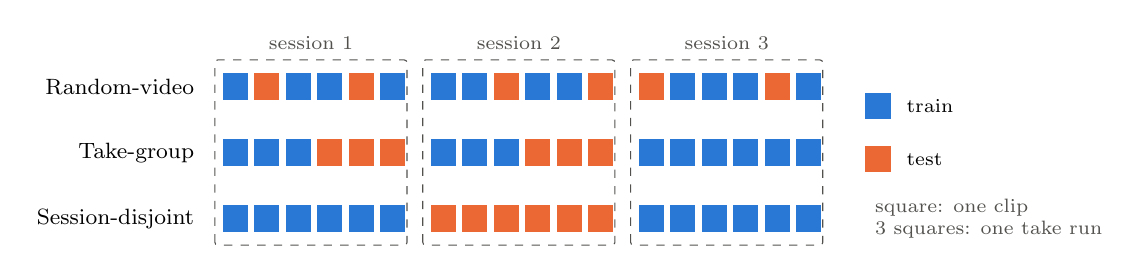
\begin{tikzpicture}[x=4.0mm, y=4.2mm]
\newcommand{\cliprow}[3]{%
  \node[anchor=east, font=\footnotesize, align=right] at (-0.6,#1) {#2};
  \foreach \i/\c in {#3} {\fill[\c] (\i,#1-0.4) rectangle (\i+0.8,#1+0.4);}
}
\foreach \x/\n in {0/1, 6.6/2, 13.2/3} {
  \draw[ink2, dashed, rounded corners=1pt] (\x-0.25,-2.8) rectangle (\x+5.85,2.8);
  \node[font=\scriptsize, text=ink2] at (\x+2.8,3.3) {session \n};
}
\cliprow{2}{Random-video}{0/cA,1/cB,2/cA,3/cA,4/cB,5/cA, 6.6/cA,7.6/cA,8.6/cB,9.6/cA,10.6/cA,11.6/cB, 13.2/cB,14.2/cA,15.2/cA,16.2/cA,17.2/cB,18.2/cA}
\cliprow{0}{Take-group}{0/cA,1/cA,2/cA,3/cB,4/cB,5/cB, 6.6/cA,7.6/cA,8.6/cA,9.6/cB,10.6/cB,11.6/cB, 13.2/cA,14.2/cA,15.2/cA,16.2/cA,17.2/cA,18.2/cA}
\cliprow{-2}{Session-disjoint}{0/cA,1/cA,2/cA,3/cA,4/cA,5/cA, 6.6/cB,7.6/cB,8.6/cB,9.6/cB,10.6/cB,11.6/cB, 13.2/cA,14.2/cA,15.2/cA,16.2/cA,17.2/cA,18.2/cA}
\fill[cA] (20.4,1.0) rectangle (21.2,1.8); \node[anchor=west, font=\scriptsize] at (21.4,1.4) {train};
\fill[cB] (20.4,-0.6) rectangle (21.2,0.2); \node[anchor=west, font=\scriptsize] at (21.4,-0.2) {test};
\node[anchor=west, font=\scriptsize, text=ink2, align=left] at (20.4,-2.0) {square: one clip\\3 squares: one take run};
\end{tikzpicture}}
\caption{Three split protocols on the same recordings (schematic). A session contains several words, and the signer records each word as a run of near-identical takes. Random-video splits put takes of one run on both sides; take-group splits keep a run together but let one session supply both training and test clips; session-disjoint splits hold out whole sessions.}\label{fig:protocols}
\src{Counts from the split definitions: the 262-word random-video split has 666 take-groups on both sides of the train/test boundary, the take-group split has all 13 session blocks on both sides, and the session-disjoint splits used for the final models have none.}
\end{widefigure}

For final models, the validation clips (taken from training sessions at take-group granularity) are folded back into training, giving 2,845 training clips over 262 words. The held-out blocks contain 1,412 clips: 1,010 form the test set, and 402 belong to words with fewer than six training clips and are marked unused. The deployed test set is the 472 test clips of the 50 deployed words, and every main result scores exactly these clips.

\paragraph{Official split.} For comparison with published results, the released configuration is also trained on the split shipped with INCLUDE, read from the dataset's distribution files and filtered to each benchmark: 675 training, 77 validation and 191 test clips for INCLUDE-50, and 3,101, 340 and 816 for the 262 words. INCLUDE-50 shares 21 of its 50 words with the deployed vocabulary. Training uses the official training clips only; the validation clips are scored every 50 epochs for monitoring and never select a checkpoint, and the final weights are kept as in Section~\ref{sec:method:train}. Each benchmark needs its own model, because 144 of the 191 INCLUDE-50 test clips are training clips of the 262-word split. Neither split separates recordings: 184 of the 191 INCLUDE-50 test clips and 767 of the 816 262-word test clips share a take-group with a training clip, and every session block supplies clips to both sides.

\subsection{Metrics, test-time views and statistics}\label{sec:method:metrics}
Top-1 and top-5 accuracy are the share of clips whose true word is ranked first or within the first five; balanced accuracy is the mean per-word recall. Unless stated otherwise, predictions follow Eq.~\eqref{eq:mask}, restricted to the 50 deployed words; unrestricted figures take the argmax over all 262 outputs. Test-time augmentation (TTA) averages softmax probabilities over six views: three temporal phases (0.25, 0.5 and 0.75 of each sampling segment), each with and without a horizontal flip that swaps the hand streams. Each main result is the mean of three seeds. Paired comparisons on identical clips use the exact two-sided McNemar test~\cite{mcnemar1947} on the discordant clips, per seed and pooled over seeds. Five seeds of one earlier configuration gave a top-1 standard deviation of 1.9 points on 1,010 clips; differences below about 5 points between single runs are therefore read as seed noise.

\subsection{Software and hardware}
Experiments ran on one desktop: NVIDIA GeForce RTX 3060 (12\,GB), AMD Ryzen 5 5500, 32\,GB RAM, Windows 11, Python 3.11.15, PyTorch 2.6.0 with CUDA 12.4, MediaPipe 1.0.0 (Tasks API), timm 1.0.28 and OpenCV. Training seeds were 0, 1 and 2; split construction used seed 1337.

% ===========================================================================
\subsection{Experimental setup}\label{sec:setup}
% ===========================================================================

Supplementary Table~\ref{tab:setup} lists the settings of the principal experiments. Results in Sections~\ref{sec:res:main} to~\ref{sec:res:perclass} use the same 472 test clips unless the table says otherwise. The launch script and result files for every experiment are listed in Supplementary Section~\ref{app:trace}.

% ===========================================================================
\paragraph{Use of AI tools.} Claude (Anthropic) assisted with writing and reviewing code and with editing the manuscript text; the authors checked all results and take full responsibility for the content.

\section{Results and discussion}\label{sec:results}
% ===========================================================================

\subsection{Main result}\label{sec:res:main}

The released 4-bit landmark model reached 85.9\% top-1 (seeds 84.5, 87.5 and 85.8), 96.4\% top-5 and 85.8\% balanced accuracy, with predictions restricted to the 50 deployed words and six-view TTA on the 472 held-out-session test clips and averaged over three independently trained seeds. Answering from all 262 words gives 72.0\% top-1 (69.7, 75.8, 70.3) and 92.7\% top-5 on the same clips; a single centre view with the mask gives 85.5\%; on the full 262-word test set (1,010 clips, single view) the same models reach 64.7\% top-1. Re-scoring the three released model files on the same test clips reproduced the stored per-clip outcomes exactly for all three seeds.

\subsection{Model variants}\label{sec:res:variants}

The variants compared here share one architecture and differ in input streams, numerical precision, temporal length or preprocessing, so each comparison isolates one change. Table~\ref{tab:variants} and Supplementary Fig.~\ref{fig:variants} compare the four variants that share the test set, the training data and the training procedure.

\begin{widetable}[t]
\caption{Controlled variants on the 472 held-out clips (50-word restriction, 6-view TTA, mean of three seeds). Each row differs from the one above in a single factor.}\label{tab:variants}
\footnotesize
\setlength{\tabcolsep}{4pt}
\begin{tabular*}{\textwidth}{@{\extracolsep\fill}llrrrrr@{}}
\toprule
Variant & Precision & Parameters & Stored size & Top-1 & Top-5 & Balanced \\
\midrule
Pixels only & FP32 & 3,803,206 & 15.2\,MB$^{a}$ & 73.7 & 93.5 & 73.3 \\
Pixels + landmarks & FP32 & 3,894,214 & 15.6\,MB$^{a}$ & 86.5 & 96.5 & 86.5 \\
Landmarks, PTQ & INT4, group 128 & 3,894,214 & as QAT & 83.4 & 95.8 & 83.3 \\
Landmarks, QAT (released) & INT4, group 128 & 3,894,214 & 2,069,700\,B & 85.9 & 96.4 & 85.8 \\
\botrule
\end{tabular*}
\src{Per-seed top-1: pixels only 75.0/73.7/72.2; landmarks 87.3/86.9/85.4; PTQ 83.1/85.2/82.0; QAT 84.5/87.5/85.8. $^{a}$Parameters $\times$ 4 bytes. 2,069,700\,B = 1.974\,MiB = 2.07\,MB.}
\end{widetable}

\paragraph{Landmark stream.} Adding the landmark stream, with nothing else changed, raised top-1 from 73.7\% to 86.5\%. The gain replicated in every seed: 76, 83 and 88 clips gained against 18, 21 and 26 lost ($p=1.2\times10^{-9}$, $6.7\times10^{-10}$ and $4.6\times10^{-9}$). The pipeline already ran MediaPipe to place crop boxes; the landmark model uses joints that the pixel-only model discarded.

\paragraph{Quantisation.} Rounding the FP32 landmark weights to 4 bits after training gave 83.4\%; quantisation-aware training reached 85.9\%. Pooled over seeds, QAT gained 77 clips and lost 41 relative to PTQ ($p=0.0012$). Against FP32, QAT gained 37 clips and lost 45 (pooled $p=0.44$): the released 4-bit model matches its FP32 version within seed noise.

\paragraph{Compute and latency.} Table~\ref{tab:runtime} reports measurements made for this paper. A forward pass of the model took \LATMS\ per view on the central processing unit (CPU).

\begin{widetable}[t]
\caption{Compute and runtime of the released model, measured on the desktop described in Section~\ref{sec:method}.}\label{tab:runtime}
\footnotesize
\setlength{\tabcolsep}{4pt}
\begin{tabularx}{\textwidth}{@{}L{3.4cm}L{2.7cm}Y@{}}
\toprule
Quantity & Value & Timing boundary and method \\
\midrule
Parameters (landmark model, 262 outputs) & 3,894,214 & counted on the instantiated network; spatial encoder 1,930,944, temporal blocks 1,779,456, landmark projections 91,008 \\\addlinespace[2.5pt]
Multiply--accumulates per view & 1.65\,G (16 frames); 0.82\,G (8 frames) & \texttt{torch.utils.flop\_counter}; matrix products and convolutions only \\\addlinespace[2.5pt]
Model forward pass, one view, CPU & \LATMS\ median (interquartile range \LATIQR) & released model (seed 0), batch 1, FP32 arithmetic, 6 threads, 100 runs after warm-up, idle machine \\
\botrule
\end{tabularx}
\end{widetable}

\subsection{Effect of the split protocol}\label{sec:res:protocol}

\begin{widefigure}[t]
\centering
\includegraphics[width=\textwidth]{figures/fig_protocol.pdf}
\caption{Accuracy of one configuration under different split protocols. (a) A 50-word pixel-only configuration (16 frames, 2,000 epochs, iSign initialisation) trained on a random-video split and on the session-disjoint split. (b) An early 8-frame, 262-word configuration trained on three splits. Labels give each protocol's test-set size $n$.}\label{fig:protocol}
\end{widefigure}

The matched 50-word comparison (Fig.~\ref{fig:protocol}a) gave 98.5\% on the random-video split (one seed, 200 clips) and 70.1\% on held-out sessions (69.9\% and 70.3\%, two seeds, 472 clips), a gap of 28.4 points. With the early 8-frame configuration on 262 words (Fig.~\ref{fig:protocol}b), accuracy fell from 94.5\% (random-video) to 29.3\% (take-group) and 22.1\% (session-disjoint). The random-video score is mostly recognition of the recording: the take-group step removes near-duplicate takes and the session step removes shared recording conditions.

\subsection{Comparison with published methods}\label{sec:res:sota}

On INCLUDE's own split, the test clips behind the published figures, the released configuration scores above each published INCLUDE result in Table~\ref{tab:sota}. Trained on the 675 official training clips of INCLUDE-50 and scored on its 191 test clips (Section~\ref{sec:method:eval}), the FP32 model reached 97.9\% top-1 with and without six-view TTA, 3.4 points above the 94.5\% reported for INCLUDE-50~\cite{sridhar2020include}; after 300 epochs of QAT the INT4 model scored 97.4\% single view and 97.9\% with TTA. Trained on the 3,101 official training clips of the 262 words and scored on the 816 official test clips present in this copy of INCLUDE, the FP32 model reached 98.8\% with and without TTA: 13.2 points above the INCLUDE baseline (85.6\%), 5.3 points above the OpenHands SL-GCN (93.5\%), 4.1 points above OpenHands with self-supervised pretraining (94.7\%)~\cite{selvaraj2022openhands} and 1.0 point above HWGAT with pretraining (97.79\%)~\cite{patra2024hwgat}. The INT4 model scored 98.8\% single view and 98.5\% with TTA.

The official split does not hold out recordings (Section~\ref{sec:method:eval}), so its scores sit with the random-video figures of Section~\ref{sec:res:protocol} (98.5\% and 94.5\%), not with held-out sessions. ISL-ViT-Tiny is the only entry in the table evaluated on held-out recording sessions; there the released model scores 85.9\% on the 50 deployed words and 64.7\% on all 262. The fall from 98.8\% to 64.7\% on 262 words is not a clean measure of leakage, because the two models also differ in training and test clips, and on 50 words the vocabularies differ as well (21 words shared). The matched measurement, about 28 points for one configuration, is the one in Section~\ref{sec:res:protocol}.

The released model is also small for what it holds: 3.89\,M parameters in 2.07\,MB. That is more than 1.4 times the parameters of TinyMSLR (fewer than 2.7\,M) in less than a third of its storage (7.2\,MB), for 50 deployed words against TinyMSLR's 20 classes. Only the Kannada models are smaller on disk (1,098\,KB); they recognise 33 words from landmarks alone, without image input.

\begin{table*}[t]
\caption{Comparison with prior isolated-sign recognisers. Top-1 accuracy (\%) is as reported by each source; corpus, vocabulary and split differ between rows.}\label{tab:sota}
\scriptsize
\setlength{\tabcolsep}{3pt}
\begin{tabularx}{\textwidth}{@{}L{3.9cm}L{2.6cm}YL{2.4cm}L{2.0cm}L{1.6cm}@{}}
\toprule
Method & Input & Corpus, words & Split & Top-1 & Size \\
\midrule
\multicolumn{6}{@{}l}{\textit{Same corpus (INCLUDE)}} \\
INCLUDE baseline~\cite{sridhar2020include} & RGB video & INCLUDE, 263 & dataset split & 85.6 & -- \\\addlinespace[2.5pt]
INCLUDE baseline~\cite{sridhar2020include} & RGB video & INCLUDE-50 & dataset split & 94.5 & -- \\\addlinespace[2.5pt]
OpenHands SL-GCN~\cite{selvaraj2022openhands} & pose keypoints & INCLUDE, 263 & dataset split & 93.5 & -- \\\addlinespace[2.5pt]
OpenHands, pretrained~\cite{selvaraj2022openhands} & pose keypoints & INCLUDE, 263 & dataset split & 94.7 & -- \\\addlinespace[2.5pt]
HWGAT~\cite{patra2024hwgat} & pose keypoints & INCLUDE, 263 & dataset split & 97.67 & -- \\\addlinespace[2.5pt]
HWGAT, pretrained~\cite{patra2024hwgat} & pose keypoints & INCLUDE, 263 & dataset split & 97.79 & -- \\\addlinespace[2.5pt]
This work, FP32 & crops, landmarks & INCLUDE-50 & dataset split & \textbf{97.9} & -- \\\addlinespace[2.5pt]
This work, INT4 & crops, landmarks & INCLUDE-50 & dataset split & \textbf{97.9} & -- \\\addlinespace[2.5pt]
This work, FP32 & crops, landmarks & INCLUDE, 262 & dataset split & \textbf{98.8} & -- \\\addlinespace[2.5pt]
This work, INT4 & crops, landmarks & INCLUDE, 262 & dataset split & \textbf{98.5} & -- \\\addlinespace[2.5pt]
This work, INT4 & crops, landmarks & INCLUDE, 262 & held-out sessions & \textbf{64.7} & \textbf{2.07\,MB} \\\addlinespace[2.5pt]
This work, INT4 & crops, landmarks & INCLUDE, 50 deployed & held-out sessions & \textbf{85.9} & \textbf{2.07\,MB} \\
\midrule
\multicolumn{6}{@{}l}{\textit{Other corpora}} \\
SPOTER~\cite{bohacek2022spoter} & 2D pose & WLASL100 & dataset split & 63.18 & -- \\\addlinespace[2.5pt]
SAM-SLR~\cite{jiang2021samslr} & skeleton, RGB, depth & AUTSL, 226 & signer-independent & 98.42$^{a}$ & -- \\\addlinespace[2.5pt]
TinyMSLR~\cite{lamaakal2026tinymslr} & RGB & PHOENIX-2014T and CSL, 20 & signer-independent & 99.01$^{b}$ & 7.2\,MB \\\addlinespace[2.5pt]
Kannada study~\cite{venkatappa2026kannada} & MediaPipe landmarks & Kannada Sign Language, 33 & -- & 94.19 to 95.71 & 1,098\,KB \\
\botrule
\end{tabularx}
\src{$^{a}$RGB track of the challenge. $^{b}$Validation accuracy. Size is given where the source states it. The dataset-split rows of this work are seed 0 with six-view TTA on the official test clips (191 for INCLUDE-50; 816 for 262 words); those models have the released architecture with a 50- or 262-word output layer. The held-out-session INT4 rows are the released model: the 262-word row is single view on 1,010 clips, and the 50-word row is the main result, restricted to the deployed words, with six-view TTA on 472 clips of the deployed words. The copy of INCLUDE used here has 262 usable words.}
\end{table*}

\subsection{Temporal length, resolution and training budget}\label{sec:res:ablation}

Going from 8 to 16 frames (Supplementary Fig.~\ref{fig:ablation}a) raised single-view top-1 from 60.0\% to 70.1\% (two-seed mean); 24 and 32 frames gave 69.7\% and 72.5\% from one seed each, within seed noise of the 16-frame result, so the model uses 16 frames at half the inference cost of 32. Crop size is set at 64 pixels (Supplementary Fig.~\ref{fig:ablation}b): 64, 112 and 128 pixels gave 46.5\%, 46.5\% and 44.0\% at 0.82, 2.34 and 3.03 giga multiply--accumulate operations (GMACs) per view. On 50 words, with a training split that also contained 76 CISLR clips and the same 472 test clips, extending training from 250 to 2,000 epochs raised top-1 by 7.9 points (two runs each); at 16 frames training length has saturated, a 4,000-epoch run gaining 0.6 points over 2,000.

\subsection{Per-word behaviour}\label{sec:res:perclass}

Twenty-seven of the 50 words reached at least 90\% recall (Supplementary Fig.~\ref{fig:perclass}). The words with the lowest recall form visually similar groups, for example \emph{big}/\emph{wide}/\emph{narrow} and \emph{good}/\emph{bad}/\emph{wet}, which differ mainly in movement or in the relation between the two hands. Top-5 accuracy on the same clips is 96.4\%.

\subsection{Cross-corpus test}\label{sec:res:cross}
The three released models were scored on CISLR without any retraining, with landmarks extracted by the same pipeline. On the 98 CISLR clips of deployed words, with the 50-word restriction, top-1 was 29.3\% (29.6, 27.6, 30.6; chance 2\%) and top-5 46.3\%; answering from all 262 words on all 609 clips, top-1 was 9.6\% (9.5, 8.7, 10.5) and top-5 22.4\%. CISLR is recorded at 300 pixels by different signers, rooms and cameras, and MediaPipe finds a genuine left hand in 25.0\% of its frames against 92.0\% on the INCLUDE test clips, so the recogniser operates on far fewer detected hands there.

\subsection{Super-resolution and the GAN}\label{sec:res:gan}

\begin{widefigure}[!t]
\centering
\includegraphics[width=0.9\textwidth]{figures/fig_gan.pdf}
\caption{Learned upscaling versus bicubic, and each GAN versus the same generator without the adversarial loss. (a) Mean top-1 of the three frozen released models on the 472 test clips after each front end; dashed lines are generators trained without an adversarial loss, and clean 1080p is the main result, 85.9\%. (b) Change in top-1 when the adversarial loss is added to an otherwise identical generator: diamonds are three-seed means, dots individual seeds, and $p$ is the pooled exact McNemar test.}\label{fig:ganres}
\end{widefigure}

Every learned upscaler beat bicubic at every resolution (Fig.~\ref{fig:ganres}); at 180p the gain was 14.3 to 15.0 points (SR-L1: +15.0, 269 clips gained and 57 lost, $p=4.5\times10^{-34}$). The adversarial term added a further gain at 240p, where v2 over SR-L1 (+1.5 points, $p=0.022$) and v3 over its control (+2.4, $p=0.001$) both met the criterion fixed in Section~\ref{sec:method:sr}; at 180p and 360p each generator scored within about one point of its counterpart without the adversarial loss, so learned upscaling accounts for nearly all of the recovery. SR-GAN v3 found the most hands at 180p (77.6\% of frames against 68.2\% for SR-L1; Supplementary Fig.~\ref{fig:exdetect}). In line with the perception--distortion trade-off~\cite{blau2018pd}, the GANs produced sharper patches with lower PSNR than SR-L1.

After the classifiers were fine-tuned for 150 epochs on 360p video through each front end, the GAN front ends reached 77.8\% (v1) and 76.9\% (v2) at 180p against 64.4\% for bicubic. A 2$\times$2 decomposition at 180p with SR-GAN v2, crossing clean or degraded pixels with clean or degraded landmarks, attributed 7.7 of the 10.5 points between the 180p and the clean result to degraded landmarks and 2.9 to degraded pixels, which locates the remaining headroom in hand-joint quality rather than in pixel texture.

\subsection{Discussion and originality}\label{sec:discussion}
% ===========================================================================

\paragraph{What moved accuracy.} The largest single gain came from an input the pipeline already computed: hand joints added 12.8 points for 91,008 parameters. Doubling the frames from 8 to 16 added about 10 points. On an earlier 50-word training split, 2,000 epochs instead of 250 added 7.9 points, but at 16 frames a further 2,000 epochs added only 0.6. With about 11 training clips per deployed word (571 clips for 50 words), explicit handshape measurements probably give the network information that 64-pixel crops carry only implicitly, which is consistent with larger crops adding tokens without adding accuracy.

\paragraph{What compression costs.} Group-wise 4-bit storage reduces the weights from about 15.6\,MB to 2.07\,MB. Rounding after training gave 83.4\%; training with the rounding in the loop gave 85.9\%, level with the FP32 model within seed noise. The 4-bit file is a storage format: its weights are expanded back to FP32 when the model is loaded.

\paragraph{What the protocol changes.} A 28-point gap between random-video and session-disjoint splits for one configuration suggests that INCLUDE accuracies reported on random splits largely measure recognition within recording sessions. INCLUDE's own split mixes recordings in the same way, and on it the released configuration scores above the published results (Table~\ref{tab:sota}). Published INCLUDE numbers~\cite{sridhar2020include,selvaraj2022openhands,patra2024hwgat} are therefore closer in kind to those official-split scores than to the 85.9\% measured here on held-out sessions, which answers a harder question than any entry in the table.

\paragraph{What the GAN study shows.} Learned upscaling recovered most of the accuracy lost at 180p, and the adversarial term added a measurable gain at 240p. The 2$\times$2 decomposition shows where the remaining headroom is: after upscaling, most of the gap to clean video lies in where the detector places hand joints. This motivated the v3 generator, trained against a hand-landmark loss, and it raised the share of detected hands at 180p from 68.2\% to 77.6\%.

\paragraph{Limitations.} All main results come from one INCLUDE test set of 472 clips over 50 words, with three seeds per variant. Recording sessions were reconstructed from camera capture counters rather than taken from dataset metadata. INCLUDE carries no signer identifiers, so a held-out session may include a signer who also appears in training sessions; the CISLR test, recorded by other signers, is the only measurement on signers outside the training data. Latency was measured on a desktop CPU, not the target wearable.

\paragraph{Originality.} This work contributes a compact recogniser built to a fixed storage budget and an evaluation built around how INCLUDE was recorded. The model reads hand and face crops and the hand-joint coordinates in one token stream, so the joints that the detector already computes cost 91,008 parameters rather than a separate pose network, and they raise top-1 accuracy by 12.8 points. Quantisation-aware training brings the complete model to 2.07\,MB at 4 bits, level with its full-precision version within seed noise. The evaluation holds out whole recording sessions, measures how much a random split inflates accuracy on this corpus, compares the same configuration with published results on INCLUDE's own split, and scores the released model on CISLR, recorded by other signers with other cameras. The super-resolution study separates the gain from a learned upscaler from the further gain added by the adversarial loss. Each of these results comes from comparisons repeated over three seeds on one fixed test set, and Supplementary Table~\ref{tab:contrib} links each contribution to its evidence and to the closest prior approach. Among the works reviewed in Section~\ref{sec:related}, we found no ISL word recogniser that reports this combination.

% ===========================================================================
\section{Conclusion and future work}\label{sec:conclusion}
% ===========================================================================

The objective of this work was an isolated-word ISL recogniser small enough for a wearable device, sized to a 2\,MB storage budget, whose accuracy is measured on recording sessions held out from training. The released model reaches 85.9\% top-1 on 50 deployed words from held-out INCLUDE sessions in a 2,069,700-byte 4-bit file. Trained on INCLUDE's own split, the same configuration scores 97.9\% on INCLUDE-50 and 98.8\% on 262 words, above the previously reported 94.5\% and 85.6 to 97.8\%. Each design choice rests on controlled comparisons on one fixed test set with three seeds. Three next steps extend the work: record the planned signer-disjoint set (three signers, 50 words, three takes) and score the released model on it unchanged; train a pose-only graph network on the same split as a second architecture family; and run the model with integer kernels on a phone-class processor, timing the detector and the classifier separately.

\backmatter

\bmhead{Acknowledgements}
The authors gratefully acknowledge Amrita Vishwa Vidyapeetham, Coimbatore, for its institutional support and facilitation of open-access publishing opportunities through Springer Nature. Figures elsewhere in the repository that show INCLUDE frames carry the dataset's CC-BY-4.0 attribution.

\section*{Declarations}

\bmhead{Code availability}
All code, configurations, split definitions, result files and the three released models are in the public repository \url{https://github.com/not-good-keeper/compact-vit-sign-language}. The launch scripts and result files of every experiment are listed in Supplementary Section~\ref{app:trace}, at commit \texttt{v1.0}.

\bmhead{Data availability}
INCLUDE (Zenodo record 4010759), CISLR and iSign are available from their authors. The repository does not redistribute video.

\bmhead{Author contributions}
N.K.K. developed the vision transformer methodology, implemented the model and its training pipeline, conducted the corresponding experiments, analysed the results and prepared the associated figures. Y.K. designed and conducted the GAN-based super-resolution study, including its implementation, experiments, analysis and figures. D.R.M. independently verified the reported results and validated the model across multiple computing platforms. B.T. supervised the project and critically reviewed the manuscript.

\bmhead{Competing interests}
The authors declare no competing interests.

\bmhead{Funding}
This work received no external funding.



\bibliography{references}

\end{document}
